\section{课程简介}

\subsection{学什么}

\begin{itemize}
	  \item {\bf Wikipedia——微积分} 
	\begin{itemize}
	  \item Latin, {\it a small stone used for counting}  
	  \item {\it a branch of mathematics focused on \underline{limits, functions,
	  	derivatives, integrals, and infinite series}} 
  	  \item {\it widespread application in \underline{science, economics,} 
  	  and \underline{engineering}} 
% 		  \item {\it constitues a major part of modern mathematics} 
	\end{itemize}
	\item {\bf John von Neumann} ({\small\it The Mathematician, 1947})
	\begin{itemize}
	  \item {\it The calculus was the \underline{first achievement} of modern
	  mathematics, and it is difficult to overestimate its importance.}
	\end{itemize} 
\end{itemize}

\begin{center}
	\scalebox{0.3}{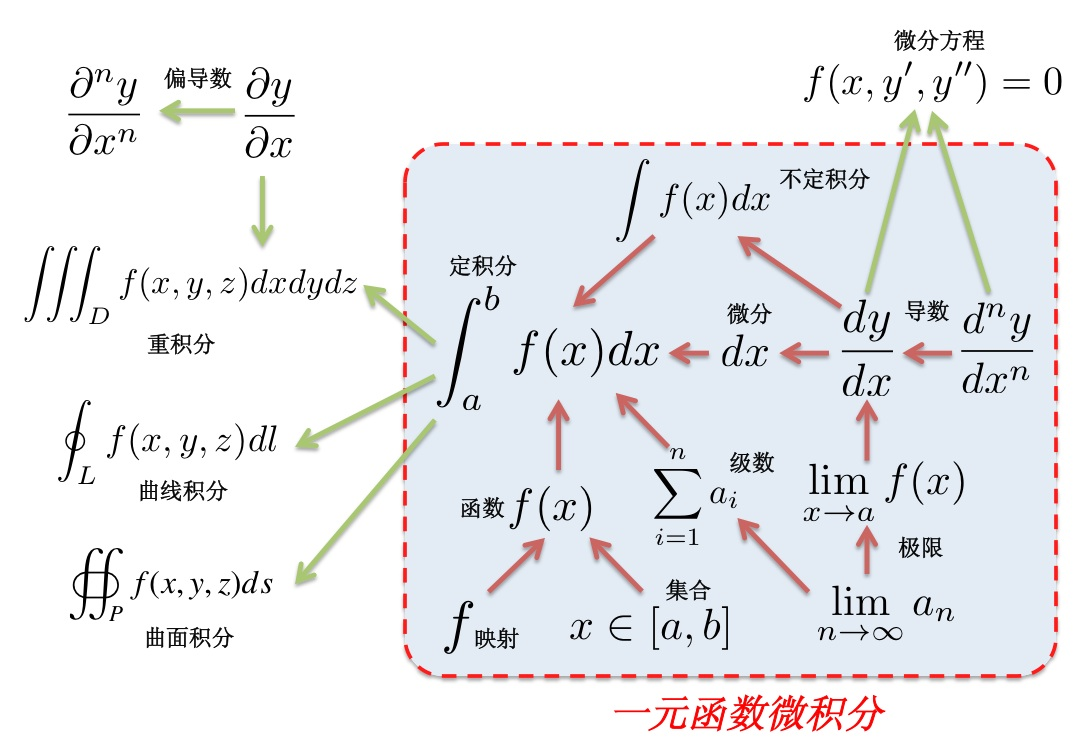
\includegraphics{./images/ch1/AM_architecture.jpg}}
% 	\ps{上课前画好}
\end{center}

\subsection{为什么学}

\begin{shaded}
	{\bf 知乎:学数学有什么好处?我们为什么要学数学?}
	\begin{itemize}
	  \item Engles:{\it 数学是一门研究现实世界的数量关系和空间形式的科学。}数学具有:
	  抽象性、精确性和应用的广泛性
	  \item Marx:{\it 一种科学只有在成功运用数学时,才算达到了真正完善的地步。}
	  \item Galileo:{\it “数学符号就是上帝用来书写自然这一伟大著作的统一语言,
	  不了解这些文字就不可能懂得自然的统一语言,只有用数学概念和公式所表达的物理世界
	  的性质才可认识……”}
	  \item Gauss:{数学是科学的女王}
	  \item 韩寒:{\it
	  我们生活中用到的数学估计到小学三年级就已经够用了。}然而在之后我们多年来学习的数学,
	  实际上塑造了我们一种理性的、条理的、系统化的思维方式。这种思维方式在我们解决自己
	  一生中遇到的诸多问题时,都有非常重要的作用。比如慎密的思考、分类的思想、排序的思想等。
	  很多东西其实都带有学习数学这个过程产生的影响,只是由于其作用方式非常隐晦,
	  也不容易被追溯其源头,我们平时不容易注意到罢了。
	  \item 王小波:{\it 我上大学时,有一次我的数学教授在课堂上讲到:我现在所教的数学,
	  你们也许一声都用不到,但我还要教,因为这些知识是好的,应该让你们知道。”}
	  \item 崔钢:{\it 1,用通用简洁的方式来表达自然规律。2,提供一些问题的分析手段。
	  3,提供认识世界的一种模式。4,了解自己的智力水平。.}
	\end{itemize}
	{\bf 豆瓣:为什么没人喜欢学习高等数学?木遥}
	\begin{itemize}
	  \item {\it 我完全不能理解,一个非数学或物理专业的学生怎么可能从这样的教育中获得一丝一毫的教益?
	  他怎么可能不发自内心地痛恨这门课程,然后在考完试之后的一个小时之内把所有内容忘得精光?
	  象三角代换这类积分技巧,不要说一个普通的心理学或者经济学专业的学生一辈子都用不到,
	  就连我也一辈子都用不到。就算在极其罕见的情形下需要求解这类问题,也完全可以求助于
	  wolframalpha.com 或者类似的工具。在我看来,在二十一世纪还要求一个普通学生手算积分,
	  就像是要求一个汽车驾校学员一定要从骑马学起一样。}
	  \item {\it \ldots一本基于数学家思维方式写出来的教材,亦即在每一个课题上从最基本的定义
	  和定理开始堆砌,直到超出教材所可能涵盖的水平为止}
	  \item {\it 如果是我来编写大学数学教材,我会争取让每一个在大学里读过数学课的人都能回答这样的问题:
	  为什么人们能精确预测几十年后的日食,却没法精确预测明天的天气;为什么人们可以通过 https 
	  安全地浏览网页而不会被监听;为什么全球变暖的速度超过一个界限就变得不可逆了;
	  为什么把文本文件压缩成 zip 体积会减少很多,而 mp3 文件压缩成 zip 大小却几乎不变;
	  民生统计指标到底应该采用平均数还是中位数;当人们说两种乐器声音的音高相同而音色不同的时候
	  到底是什么意思⋯⋯这不是什么「趣味数学」,这就是数学。基础、重要、深刻、美的数学。}
	  \item {\it 在我的设想里,这才是大学基础数学教育所应该达成的任务。
	  不是培养一个非数学专业的现代人在数学领域的专业素质(这是无论如何也不可能成功的),
	  而是让一个人能够在非专业的前提下最大程度地掌握真正有用的现代数学知识,
	  了解数学家们的工作怎样在各个层面上和社会产生互动,以及社会在这个领域的投资得到了怎样的回报。
	  别的科学门类的基础教育也应当是这样。}
	\end{itemize}
	{\bf 知乎:学习编程及做程序员对微积分的要求高吗?}
\end{shaded}

\begin{itemize}
  \item {\bf 数学的三大功能}
  \begin{enumerate}
    \item 为学习其他知识(课程)提供数学工具
    \item 培养理性思维
    \item 弘扬数学文化
  \end{enumerate}
  \item {\bf 数学素质}
  \begin{enumerate}
    \item 从实际问题抽象出数学模型的能力
    \item 计算与分析的能力
    \item 了解和使用现代数学语言和符号的能力
    \item 使用数学软件学习和应用数学的能力
  \end{enumerate}
\end{itemize}

\subsection{怎么学}

\begin{itemize}
	\item {\bf 参考资料}
  	\begin{enumerate}
		\item {\bf 课程配套辅导}
	  	\begin{itemize}
	  	  \item 朱健民 等,高等数学(第二版,上、下),高等教育出版社,2015,北京\ps{简称:\b 教材} 
	    	\item {李建平 等,高等数学典型例题与解法(上、下),国防科技大学出版社,2009,长沙}
	    	\ps{简称:\b 辅导书} 
	  	\end{itemize}
  		\item {\bf 参考书} 
  		\begin{itemize}
	    	\item \underline{同济大学数学系,高等数学(第六版,上、下),高等教育出版社,2006,北京}
	    	\ps{简称:\b 同济}  
	    	\item 菲赫金哥尔茨,微积分学教程(第一至三卷),第8版,高等教育出版社,2006,北京 
	    	\item James Stewart, Calculus(5th eds.)(影印版,上、下册),高等教育出版社,2004,北京
	    	\item 任何有关教学内容和\underline{数学历史}的书籍
  		\end{itemize}
  		\item {\bf MOOC:}《高等数学》,朱健民\,教授\ps{简称:\b MOOC} 
	\end{enumerate}
	\item {\bf 学习方法}
% 	\begin{itemize}
% 	  		\item {\bf 听课}\dotfill {\bf 30}
% 		\begin{itemize}
% 	  		  \item 典型问题、典型方法
% 	    	  \item 师傅领进门,修行在个人
% 	 	\end{itemize}
% 	  		\item {\bf 练习}\dotfill {\bf 50}
% 	 	\begin{itemize}
% 	    		\item 熟能生巧!
% 	    		\item 记忆!琢磨!
% 	  	\end{itemize}
% 	  		\item {\bf 思考}\dotfill {\bf 20}
% 	  	\begin{itemize}
% 	    		\item 总结!
% 	    		\item 质疑!
% 	  	\end{itemize}
% 	\end{itemize}
	\begin{enumerate}
	  \item {\bf 预习:}浏览每讲的内容梗概,懂与不懂都做到心中有数
	  \item {\bf 听课:}带着问题听讲,看如何克服难点解决问题
	  \item {\bf 复习:}阅读教材,梳理每讲要点(重要概念,典型问题,典型方法),解决遗留问题
	  \ps{推荐:\b 康奈尔笔记法}\\
	  \centerline{\it 定义会说、定理会证、公式会推、例题会作}
	  \item {\bf 练习:}独立完成课后习题,重点难点问题有选择性地增加自主练习\\
	  Polya:{\it 我们的任何一门学问都由知识和技能组成。如果你对初等或高等数学的研究工作
	  的确有真正的经验的话,那么你对下述这一点将毫不怀疑:在数学中,技能比仅仅掌握
	  一些知识要重要得多。什么是技能呢?数学技能就是解题能力——不仅能解决一般的问题,
	  而且能解决需要某种程度的独立思考、判断力、独创性和想象力的问题}
	  \item {\bf 反思:}勤思多问,{\it 学会发现和提出问题比尝试解决问题更加重要}
	  \ps{“思之不得则成疑,有疑就要问!”}\\
	  \centerline{\it What$\to$How$\to$Why$\to$Why not$\to$What if}
	  \ps{Einstein:提出一个问题往往比解决一个问题更重要!}
% 	  \centerline{\it amateur$\to$expert}
	\end{enumerate}
\end{itemize}

\section{几点要求}
\begin{itemize}
	\item {\bf 课堂:安静!安静!!安静!!!}
	
	{\bf - No to}
	  \begin{itemize}
	    \item Chatting
	    \item zZZ\ldots
	    \item anything noisy
	    \item \ldots
	  \end{itemize}
	{\bf - Yes to}
  \begin{itemize}
    \item listen to me
    \item discuss {\bf with me}
    \item do sth. you like {\bf quietly}
    \item zzz\ldots
    \item leave/enter the classroom {\bf quietly}
    \item \ldots
  \end{itemize}
  \item {\bf 作业}
  \begin{itemize}
    \item 正确、规范、工整
    \item no copy !!!!
    \item 订正每一个错误!
  \end{itemize}
	\item {\bf 答疑}
	  \begin{itemize}
	    \item 有问必答
	    \item 除了问考试、问隐私
	  \end{itemize}
% 	  \item {\bf 从善如流}
\end{itemize}

\newpage

\begin{shaded}
	{\bf\Large Cornell Note-Taking System}\hfill{\it康奈尔笔记法(5R笔记法)}
	
	\bigskip
	
	{\it 这一方法几乎适用于一切讲授或阅读课,特别是对于听课笔记,5R笔记法应是最佳首选。
	这种方法是记与学,思考与运用相结合的有效方法。具体包括以下几个步骤:}
	
	\begin{center}
		\resizebox{!}{8cm}{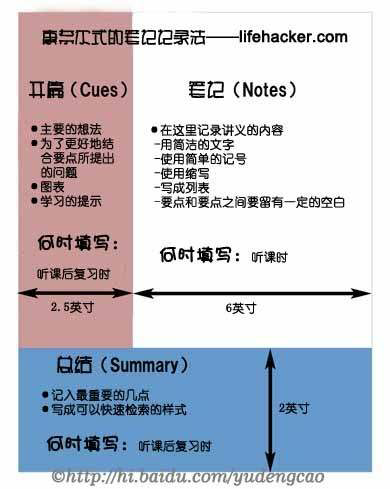
\includegraphics{./images/00/Cornell-NTS/NTS-CH.jpg}}\quad
		\resizebox{!}{8cm}{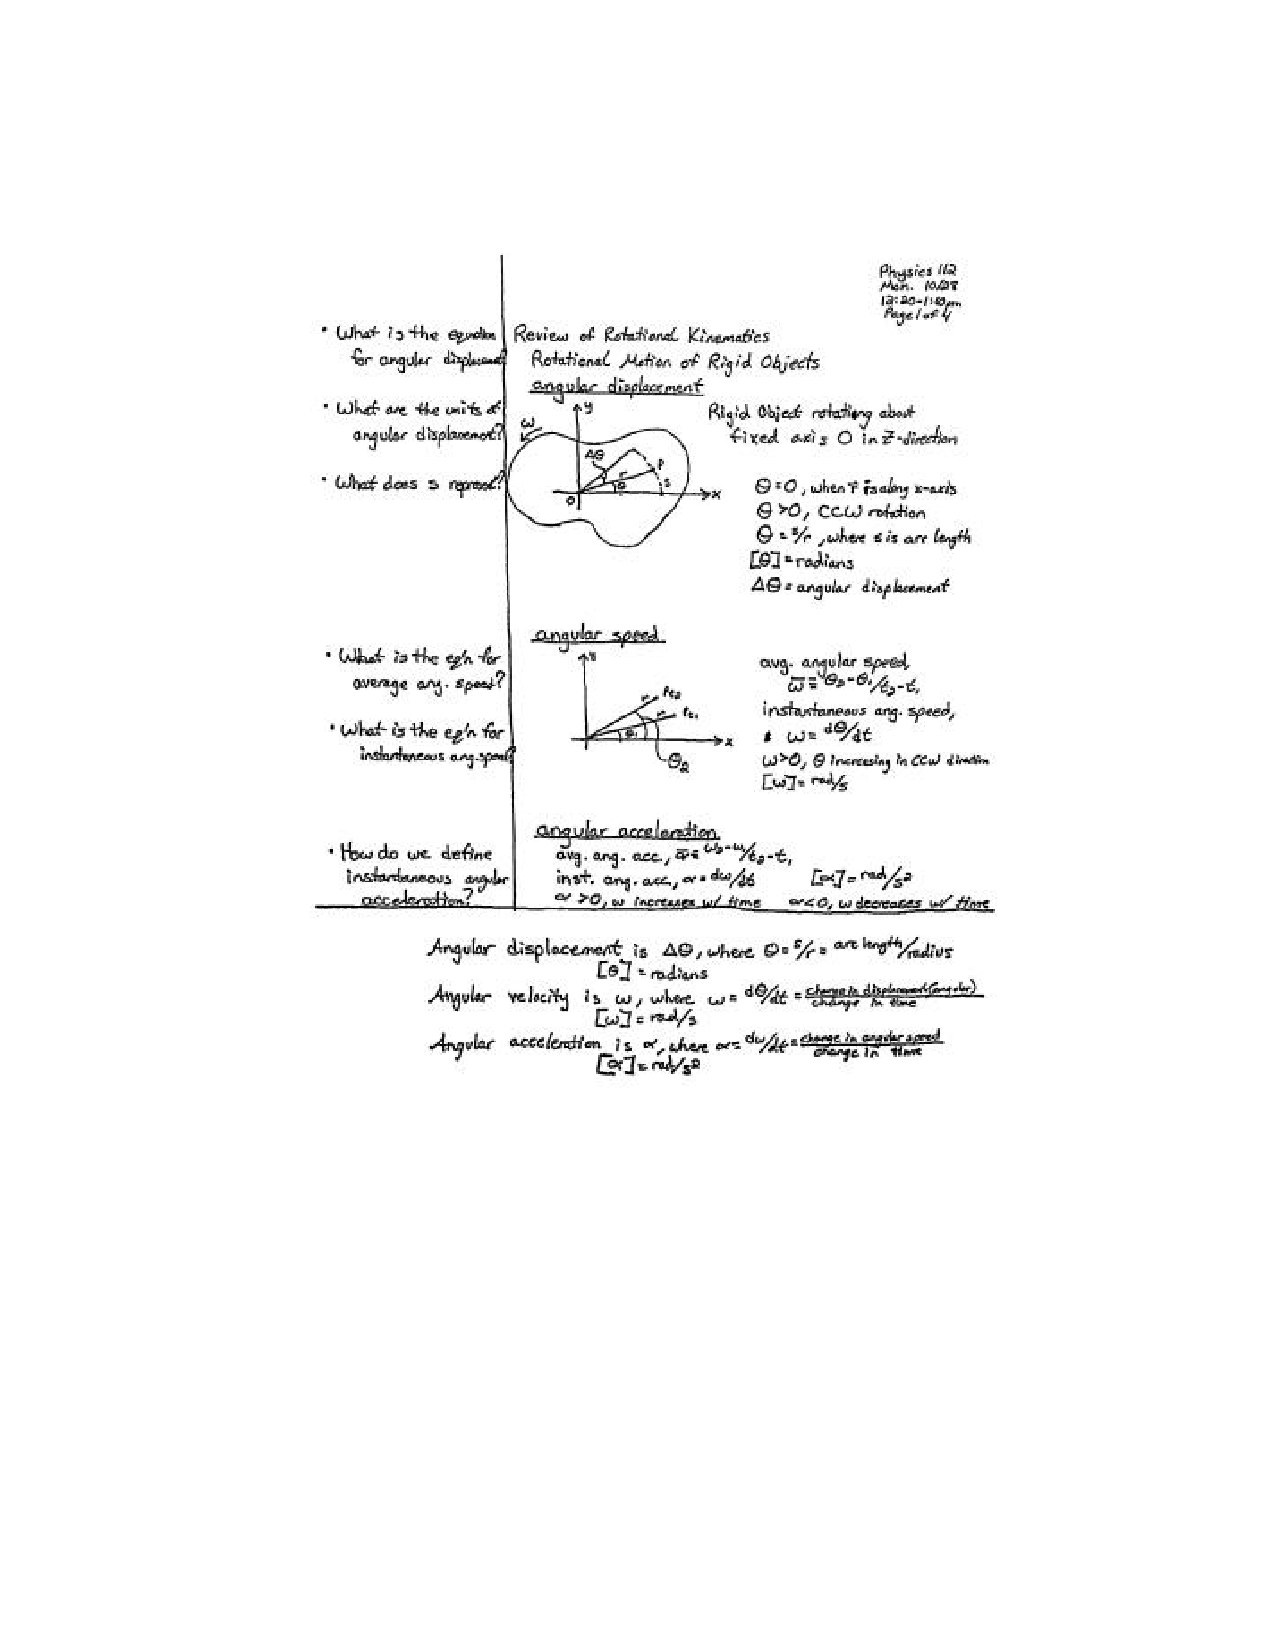
\includegraphics{./images/00/Cornell-NTS/exCNTS.pdf}}
	\end{center}
	
	\begin{enumerate}[Step1]
	  \item {\bf 记录(Record):}在听讲或阅读过程中,
	  在主栏(将笔记本的一页分为左大右小两部分,
	  左侧为主栏,右侧为副栏)内尽量多记有意义的论据、概念等讲课内容。
	  \item {\bf 简化(Reduce):}下课以后,尽可能及早将这些论据、概念简明扼要地概括(简化)
	  在回忆栏,即副栏。
	  \item {\bf 背诵(Recite):}把主栏遮住,只用回忆栏中的摘记提示,
	  尽量完满地叙述课堂上讲过的内容。
	  \item {\bf 思考(Reflect):}将自己的听课随感、意见、经验体会之类的内容,
	  与讲课内容区分开,写在卡片或笔记本的某一单独部分,加上标题和索引,
	  编制成提纲、摘要,分成类目。并随时归档。
	  \item {\bf 复习(Review):}每周花十分钟左右时间,快速复习笔记,主要是先看回忆栏,
	  适当看主栏。
	\end{enumerate}
	
	在课本、参考书原文的旁边加上各种符号(如直线、双线、黑点、圆圈、
	曲线、箭头、红线、蓝线、三角、方框、着重号、惊叹号、问号等等),便于找出重点,
	加深印象,或提出质疑。什么符号代表什么意思,你可以自己掌握,但最好形成一套比较
	稳定的符号系统。这种方法比较适合于自学笔记和预习笔记。
	
	操作时注意以下一些准则:
	{\it 读完后再做记号,要非常善于选择,用自己的话,简洁,迅速,整齐}
	
	笔记的加工:{\it 忆$\to$补$\to$改$\to$编$\to$分$\to$舍$\to$记}	
\end{shaded}

\chapter{映射与函数}

{\bf 关键词:}集合、集合论、映射、函数、曲线及其表示

\section{集合与映射}

\subsection{集合}

{\it Cantor,1874:}\ps{对于集合,“我们只需描述它,而不必给出精确的定义”}
所谓{\it 集合},是指把一些个体({\it 元素}) 放在一起考虑时它们形成的整体。
\begin{itemize}
  \item 关系符号:$\subset, \in, =, \subseteq, \neq$
  \item 运算符号:$\cap,\cup, \setminus, \bar{A}, \times, +, - $\quad ({\it
  依次为:交、并、差、补、笛卡尔积、不交并、差})
\end{itemize}
	
{\bf 常见(用)的集合:}
$\mathbb{N}\subset\mathbb{Z}\subset\mathbb{Q}\subset\mathbb{R}\subset\mathbb{C}$
\ps{\b 本书约定,自然数集包含数$0$}
	
\quad ({\it 依次为:自然数集、整数集、有理数集、有理数集和复数集})

{\bf 注:}通过集合的笛卡尔积“$\times$” 可以定义更{\it
“高维”}的集合,例如:$\mathbb{R}$表示数轴(上的所有点构成的集合),
$${\b \mathbb{R}^2=\mathbb{R}\times\mathbb{R}}$$
则表示全平面(上的所有点构成的集合)

\subsection{区间和邻域}

{\bf 例:}给定$a,b\in\mathbb{R},a<b$,区间$(a,b)=\{x\in\mathbb{R}|a<x<b\}$

{\bf 例:}记实数集$\mathbb{R}=(-\infty,+\infty)$

{\bf 注意:}{\b由于$\pm\infty$都不是具体的数,因此在本门课程中,除非特别说明,形如
\ps{\b 请对讲义中蓝色字体的部分多加留意!}
$$x=+\infty\quad\mbox{或}\quad x=-\infty$$
的写法总是错误的,而只能写
$$x\to+\infty\quad\mbox{或}\quad x\to\infty$$
}

{\bf 邻域}
$${\b U(a,\delta)}=(a-\delta,a+\delta)=\{x\in\mathbb{R}||x-a|<\delta\}$$
含义为:(实数集中所有)与$a$距离不超过$\delta$(的点构成的集合)

{\bf 例:}
$$(a,b)=U\left(\df{a+b}2,\df{b-a}2\right)$$

{\bf 去心邻域}\ps{同济写做$U^0(a,\delta)$}
$${\b
U_0(a,\delta)}=(a-\delta,a+\delta)-\{a\}=\{x\in\mathbb{R}|0<|x-a|<\delta\}$$

{\bf 无穷邻域}*\ps{名词后面加星号的,表示了解即可}
$$\{x\in\mathbb{R}||x|>M\},\;M>0$$

{\bf 问:}以上无穷邻域可以写成类似$U(\infty,M)$的形式吗?({\it 答:因为$\infty$不是一个具体的数(点),
所以为了避免误解,我们不会这么写!})

{\b 半邻域,左(右)邻域},例如:点$a$的右半邻域为
$$\{x\in\mathbb{R}|a<x<a+\delta\}$$

\ps{灰色背景内容为扩展知识,了解即可}

\begin{shaded}

{\bf 集合论、Russell Paradox与公理系统}

	{\it Cantor,1874:}朴素集合论的诞生。	

	{\it Poincare,1900,国际数学家大会:} 
		 {“\ldots 借助集合论概念,我们可以建造整个数学大厦\ldots  今天,我们可以说绝对的严格性已经达到了\ldots”}
	
	{\it Russell, 1901:}只给不给自己理发的人理发的理发师该不该给自己理发?
	
	“由所有不包含集合自身的集合所构成的集合”,记为$S$。不论$S$是不是自身的元素,按照$S$的定义都会有矛盾。
	
	设$x\in A$表示:$A$给$x$理发, 定义
	$$A=\{x|x\notin x\},$$ 
	
	问:$A\in A$还是$A\notin A$? 
	
% 	\ba{罗素悖论导致了第三次“数学危机”的出现!}
	{{\bf {第三次“数学危机”}}(Frege,1901,《算术基础》)}
		“在工作结束之后发现那大厦的基础已经动摇,对于一个科学工作者来说,没有比这更不幸的了”
		
	\begin{itemize}
	  \item {{\bf 无限抽象原则}(Cantor,Frege):} 任意给定某个条件就可以确定一个集合。(每个概念的外延可以确定一个集合)
	  \item {\bf 观点:}不加限制地使用无限抽象原则将导致罗素悖论
	  \item {{\bf 有限抽象原则}(限制公理):} 如果已知一个集合和一个给定的条件,
	  则该集合中所有满足条件的元素{\it 可以}构成一个集合。
	  \item {\bf ZF(Zermelo-Fraenkel)公理化集合论}
	  (Zermelo-Fraenkel Set Theory):包含选择公理的称ZFC,否则为ZF。
	  
	  {\bf 命题:}在ZF/ZFC中,无法定义包含所有集合的集合。
	
	{\bf 证明:}反证法。设$A$是一个这样的集合。定义
	$$B=\{x\in A|x\notin x\}$$
	若
	$B\in A$,则必有$B\in B$或$B\notin B$。而若$B\in B$,可推出$B\notin B$;同理,
	由$B\notin B$,也可推出$B\in B$。从而$B\notin A$,推出矛盾。这说明$B$的定义存在问题,故知假设错误。

	\item {\bf 公理(Axiom):}无须证明即为正确的命题。
	\begin{itemize}
	  \item {\bf Engles:}数学上的所谓公理,是数学需要用作自己出发点的少数思想上的规定 
	  \item {\bf ZFS系统:}公理就是一些关于逻辑符号{“$\in$”}和{字母}的组合使用方法的约定
	  \item {\bf 公理化方法}是构建现代数学理论体系的基石
	\end{itemize}
	\item {\bf {数学等于永恒的真理吗?}}
	\end{itemize}
	
	{\bf 注:}ZFC有无穷多个公理,因为替代公理实际上是公理模式。已知ZFC和ZF集合论
	二者都不能用有限数目个公理来公式化。
	
	{\bf 讨论:}公理(Axiom)、定理(Theorem)、定律(Law)、假设(Assumption)、
	引理(Lemma)、推论(Corallary)、猜想(conjuction)有何异同?
	
	{\it 试答:这些概念都是对规律或规则的表达。
	
	公理是数学及其相近领域所使用的概念,即在数学理论体系中无须证明即视为正确的命题(例如:
	两点之间直线最短),是数学理论体系的出发点。通过推理和演绎,我们可以在公理的基础上
	进一步推出新的结论,这些结论我们通常称为定理,引理和推论则是定理推导的中间和后续结果。
	使用不同的公理作为出发点,可能得到完全不同的理论体系,例如:非欧几何的多条基本公设(公理
	的另一种说法)就是和欧式几何不同的,这导致二者的理论体系看起来大相径庭。
	
	我们目前所使用的公理多数来源于生活中的直观体验,是一种对直觉观察的抽象描述。而由于
	我们对自然世界认识的局限性,这些描述本身可能是不精确甚至是不正确的。从这个意义上说,我们
	更应该说公理其实是我们对于客观规律的假定,是先验的,但也是可以有所调整和变化的。
	
	定律也具有类似的特点,因为人类总是在不断改进和加深对于自然世界的认识。定律更多
	地出现于物理、化学等非抽象领域,体现的是对自然规律的描述。定律背后通常存在一些的
	基本假定(例如:原子是不可分的、光既是例子又是波),定律的发现需要以重复实验为基础,
	定律的描述中一部分是可以用数学工具来刻画的(例如万有引力定律、质能方程)。
	
	公理、定理、定律的共性之处在于它们在各自的领域中或背景下,都被视为是“正确的”(请注意在数学中
	正确和可证明有时是被混同的),是被验证、证明或直接假定为真的命题,而猜想则是被
	猜测为真,但未经过这些过程,所以仍无法断言为真的。当今的数学界,仍有大量的猜想有待证明或证否,
	这些问题所代表的恰恰是数学的最前沿。
	}
\end{shaded}
	
\subsection{实数集的性质}
	\begin{enumerate} 
	  \item {\bf 有序性:}即任何两个实数均可以比大小\quad (注:$\mathbb{R}^2$、$\mathbb{C}$不具备有序性) 
	  \ps{$\mathbb{R}$是全序的,而$\mathbb{R}^2$、$\mathbb{C}$在一定的度量下
	  是半序的}
	  \item {\bf 完备性(连续性): }实数集与数轴上的点之间存在一一对应
	  
	  {\bf{连续性公理(确界原理):}}非空有{上界}的实数集必有{上确界} (最小的上界)\\
	  {\bf 注}:实数集的完备性更准确的说法应该是:实数集的任意非空有上界的子集都有上确界,且该上确界为实数
	\end{enumerate}
	
	为了更好地理解确界原理,必须对集合的有界性以及上(下)界和上(下)确界的概念有非常准确的理解:
	
	{\bf 上界:}$M\in\mathbb{R}$称为集合$A\subset\mathbb{R}$的上界,是指:对任意$x\in A$,均有
	$$x\leq M.$$
	
	{\bf 集合$A$有上界:}即存在$M\in\mathbb{R}$为$A$的上界\ps{显然上界是不唯一的!}
	
	{\bf 集合$A$有界:}即$A$同时有上下界
	
	{\bf 上确界:}{\b
	$M_0\in\mathbb{R}$称为集合$A\subset\mathbb{R}$的上确界(记为$M_0=\mathrm{sup}A$),
	是指:$M_0$是$A$的最小上界},也即
	\ps{准确理解上确界的概念是本章的难点!\\
	下确界记为:\b$\mathrm{inf}A$}
	\begin{enumerate}[(1)]
	  \setlength{\itemindent}{1cm}
	  \item 对任意$x\in A$,均有$x\leq M_0$
	  \item 对$A$的任意上界$M$,均有$M_0\leq M$
	\end{enumerate}
	其中(2)亦可表述为:{\b 对任意$\e>0$,都存在$x_{\e}\in A$,使得$M_0-\e<x_{\e}\leq M_0$}
	
	{\bf 注:}{\b 有理数集不满足连续性公理!}准确地说就是:有理数集的非空有上界的子集,
	其上确界未必是有理数	(但肯定是实数)!
	\ps{这里所说的完备性可以理解为,该集合对于取上确界的运算封闭}
	
	{\bf 例:}考虑集合$A=\left\{\left(1+\frac 1n\right)^n|n\in\mathbb{N}\right\}$,因为
	有理数的有限次四则运算仍是有理数,故显然$A\subset\mathbb{Q}$。如下图所示,集合$A$中的点如果按照
	$n$的大小排序,可以视为一个单调递增有上界(例如$3$使其一个上界)的数列,
	$$\left(1+\frac11\right)^1<\left(1+\frac12\right)^2<\left(1+\frac13\right)^3<\ldots
	\left(1+\frac1n\right)^n<\ldots,$$
	\begin{center}
		\resizebox{!}{5cm}{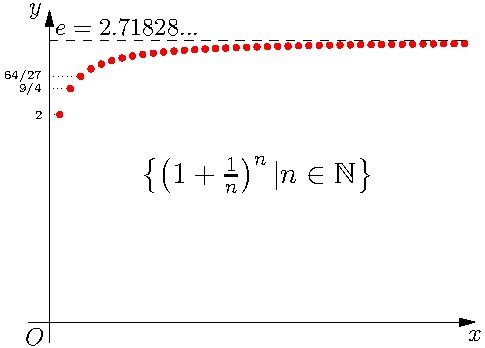
\includegraphics{./images/ch1/e-notin-N.pdf}}
% 		\resizebox{!}{4.8cm}{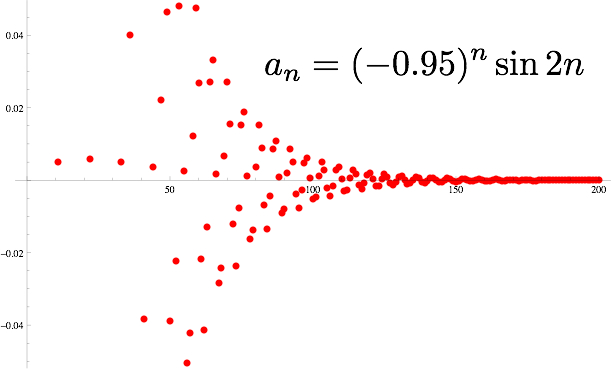
\includegraphics{./images/ch2/sin2nn.jpg}}
% 		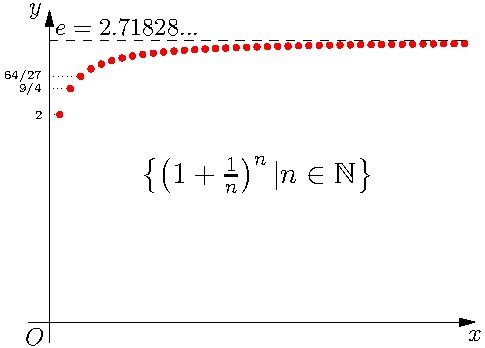
\includegraphics[width=6cm]{./images/ch1/e-notin-N}
	\end{center}
	根据常用极限
	$$e=\lim\limits_{n\to\infty}\left(1+\df1n\right)^n,$$
	不难看出$e=\mathrm{sup}A$。由于$e\notin\mathbb{Q}$,故有理数集不满足连续性公理。
	\ps{有理数集的有限次四则运算仍是有理数}
	
	{\bf 思考:}上确界和最大值有什么异同?如何确定一个集合的上确界?
	
	\begin{shaded}
	{\bf 开集与闭集}
	
	集合$A\subset\mathbb{R}$为{\bf 开集},是指:对任意$x\in A$,均存在$\delta>0$,使得
	$$U(x,\delta)\subset A.$$
	
	集合$A\subset\mathbb{R}$为{\bf 闭集},是指其补集$\bar{A}=\mathbb{R}-A$为开集。
	
	例如:所有的开区间都是开集,所有的闭区间为闭集,{\b 实数集$\mathbb{R}$既是开集又是闭集}。
	({\it 约定:空集$\phi$既是开集又是闭集})
	
	点$a$称为集合$A$的{\bf 内点},是指:存在$\delta>0$,使得$U(a,\delta)\subset A$。显然开集中的点均为其内点!
	
	点$a$称为集合$A$的{\bf 外点},是指:存在$\delta>0$,使得$U(a,\delta)\cap A=\phi$。
	
	点$a$称为集合$A$的{\bf 边界点},是指$a$既不是$A$的内点,也不是$A$的外点。
	
	显然,闭集可以视为其最大开子集和其所有边界点的并。
	
	{\bf 思考:}以下集合哪些是开集,哪些是闭集?
	\begin{enumerate}[(1)]
	  \setlength{\itemindent}{1cm}
	  \item $\{1,2,3,5\}$\quad\quad({\it 闭})
	  \item $U_0(1,3)$\quad\quad({\it 开})
	  \item 自然数集\quad\quad({\it 闭})
	  \item 有理数集\quad\quad({\it 既非开又非闭})
	  \item 无理数集\quad\quad({\it 既非开又非闭})
	  \item $\left\{\left(1+\frac
	  1n\right)^n|n\in\mathbb{N}\right\}+\{e\}$\quad\quad({\it 闭})
	\end{enumerate}
	
	\end{shaded}

\subsection{映射}

{\bf 教材:}事物之间“一对一”或“多对一”的依赖关系

{\bf 注:}将映射视为一种输入输出过程,“一对一”或“多对一”保证了
一个输入只能得到一个特定的输出,因此结果是无歧义的。从这个意义上说,对于映射
的这种定义方式也是一种约定。

$$f:A\mapsto B$$
或
$$y=f(x),\;x\in A,y\in B$$

{\bf 映射的三要素:}定义域、值域、对应关系,任何一项不明确都不足以确定一个函数,或者说,
两个映射在这三方面有一点不同,则应视为不同的映射。
\ps{之所以有时候只关心定义域和对应关系,前提是默认假设映射为满射}

{{\bf 例:}以下函数中哪些是完全相同的?}
		$$x,\quad |x|,\quad e^{\ln x},\quad \ln(e^x),\quad \sqrt{x^2},\quad
		\frac{x^2-4}{x-2}-2,$$
		$$\sin(\arcsin x),\quad \arcsin(\sin x), \quad \tan(\arctan x)$$

{\bf 相关概念:}单射、满射、一一映射(双射)

\begin{shaded}
	{\bf 一一映射与无穷集合}
	
	{\bf 问题:}如何比较两个集合中元素的个数({\it “度”})?
	
	{\bf 答:}如果存在集合$A$和$B$之间的一一映射,则称$A$和$B$是{\it 等势}的,或者说二者
	的度相同。
	
	{\bf 例:}判断正误(正确的命题须给出证明,错误的须给出证明或举反例)
	\begin{itemize}
	  \setlength{\itemindent}{1cm}
	  \item 自然数与正偶数“一样多”?({$\surd$})
	  \item 自然数与整数“一样多”?({$\surd$})
	  \item 自然数与有理数“一样多”?({$\surd$})
	  \item 区间$(a,b)$中的实数与$\mathbb{R}$中“一样多”?({$\surd$})
	  \item 自然数与实数“一样多”?({$\times$})
	\end{itemize}
		
	{\it Cantor}第一次定义了{\b{\bf 无穷集合},即:可以和自身的某个子集建立起一一映射的集合}
\end{shaded}	

	
\section{函数}
	
	\begin{shaded}
		{\bf 关于函数}
		\begin{itemize}
  		  \setlength{\itemindent}{1cm}
		  \item 微积分是关于运动和变化的数学;
		  \item 函数是对运动(例如:曲线、曲面、波以及各种变化)变化过程中各种量与量的依赖关系的抽象描述;
		  \item 函数刻画了运动变化中的量之间的相互依存关系({\bf 注:}与“依存”对应的关系叫做“独立”)
		\end{itemize}
		
		{\bf 常量和变量}
		\begin{itemize}
  		  \setlength{\itemindent}{1cm}
		  \item {\bf 常量和变量是相对的},在一定条件下可以相互转化
		  \item 变量之间的关系可能是相互依存,也可能是相互独立的
		  \item 为了避免讨论过于复杂,简化问题,我们可能选择只考虑部分参数的变化,而将其他参数视为(或设为)常量,
		  例如:万有引力与两个物体的质量、距离以及引力常数(系数)都有关,为了确定其数量关系,需要事先假定部分的参数
		  值是固定不变的
		\end{itemize}
		
		{\bf 大学数学与中学数学}
		\begin{itemize}
  		  \setlength{\itemindent}{1cm}
		  \item 数学并无严格的“高等”和“初等”之分,只是存在众多的分支和领域
		  (例如:代数、几何、分析、图论,几何又分为平面几何、立体几何、解析几何等),
		  不同分支或领域的直观性和难度各有不同
		  \item 对于函数,中学阶段更注重在对应关系“确定”的情况下,寻找其数学描述或利用给定的值进行计算
		  \item 大学阶段,从微积分开始,更着重对函数的整体特性,以及不同函数间的转换、类比和关于其整体特征的计算与分析
		\end{itemize}
		
		 {\bf James Stewart, Calculus(5th eds.), 2004}
		  \begin{itemize}
  		    \setlength{\itemindent}{1cm}
		    \item {\it Calculus is fundamentally different from the mathematics that
		    you have studied previously}
		    \item {\it Calculus is less static and more \underline{dynamic}}
		    \item {\it It is concerned with change and \underline{motion}}
		    \item {\it It deals with quantities that \underline{approach} other
		    quantities}%\marginpar{note}
		  \end{itemize}
	\end{shaded}

	{\bf (一元)函数:}由实数集到实数集的映射
	$$f:D\mapsto\mathbb{R},\;(D\subset\mathbb{R})$$
	或
	$$y=f(x),\quad (x\in D\subset\mathbb{R},y\in\mathbb{R})$$
% 	\begin{itemize}
% 	  \item {\bf 定义域:} $D\subset \mathbb{R}$ ,且$D\ne\phi$ 
% 	  \item {\bf 对应关系:} $f:D\to\mathbb{R}$
% 	\end{itemize} 
	{\bf 函数图像}
	$$G=\{(x,f(x))\in\mathbb{R}^2|x\in D\}$$
	
	\begin{shaded}
		{\bf 多元函数:} 
		$$f:D\to\mathbb{R},\quad D\in\mathbb{R}^n$$
		
		{\bf 向量值函数:}
		$$f:D\to\mathbb{R}^n,\quad, D\in\mathbb{R}$$
		
		{\bf 思考:}二元函数和三维的向量值函数对应的几何对象分别是什么?
		
	\end{shaded}	
	\begin{center}
		\resizebox{!}{4.2cm}{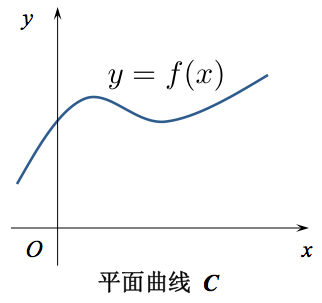
\includegraphics{./images/ch1/C_fx.jpg}}\quad	
		\resizebox{!}{4.5cm}{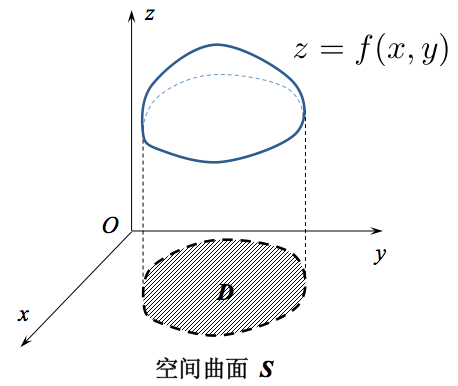
\includegraphics{./images/ch1/S_fxy.jpg}}
	\end{center}
	
	{\bf 思考:}{\b 平面曲线与一元函数具有一一对应关系吗?}空间曲面和二元函数呢?
	
	{\it 答:不是的,例如圆$x^2+y^2=1$如果写成一元函数形式,需要至少两个函数
	$y=\pm\sqrt{1-x^2}$。空间曲面和二元函数的关系与之类似。
	
	由于该问题的存在,在刻画平面曲线(空间曲面)时,我们也常常用到其他的曲线方程形式,
	例如:单位圆的方程也常常写为:
	\begin{description}
  		\setlength{\itemindent}{1cm}
		\item[隐函数方程]:$x^2+y^2=1$
		\item[参数方程]:$(x,y)=(\cos t,\sin t),\quad t\in[0,2\pi]$
		\item[极坐标方程]:$\rho=1,\theta\in[0,2\pi]$
	\end{description}
	}	
	
\subsection{函数的运算}

{\bf 基本的函数运算:}四则运算、复合运算、逆运算	
\ps{\b 如未特别说明,所列出的运算次数均为有限的,无穷次的函数四则运算和复合可能导致一些特殊的函数性质出现}

{\bf 1、四则运算:}$+,z,\cdot,/$

% {\bf 例:}$f(x),x\in A$和$g(x),x\in B$,
% $$(f\cdot g)(x)=f(x).g(x),\quad x\in A\cap B$$
% $$(f\cdot g)(x)=f(x).g(x),\quad x\in A\cap B,\;g(x)\ne 0$$
% 
% {\bf 注:}运算后函数的定义域不能以运算后的形式来确定!

{\bf 2、复合运算:}函数的复合运算就是中间变量的代入过程%,复合函数又称为函数的函数。

$$(f\circ g)(x)=f(g(x))$$

% 将复杂的函数为多个函数的复合是处理复杂的函数运算和操作(例如:求导)
% 时常用的方法!

{\bf 3、逆运算:}函数求逆(反函数)要注意反函数存在的条件:$f$为{\it 双射}

{\bf 问:}$y=f(x)$和$x=f^{-1}(y)$的图形的关系是怎样的?({\it 答:相同!})

\subsection{函数的简单性质}
	
\begin{shaded}
	{\bf 常用的简写符号:}用于数学推导中一些常用汉字的书写替代
	\begin{itemize}
	  \item {\b$\bm{\forall}$} \quad 任意 (for all)
	  \item {\b$\bm{\exists}$} \quad 存在 (exist)
	  \item {\b$\bm{\Rightarrow}$} \quad 推出 (deduce, imply)
	  \item {\b$\bm{\Leftrightarrow}$} \quad 等价、当且仅当 (equivalent, if and only if)
	  \item {\b$\bm{\to}$} \quad 趋于 (approach)
	\end{itemize}
\end{shaded}

\subsubsection{【有界性】}			

{{\bf 定义:}}
	设$I\subset\mathbb{R}$,$f(x)$在$I$上有定义,若集合
	$$\{f(x)|x\in I\}$$
	有界,则称{\it $f(x)$在$I$上有界}或{\it $f(x)$是$I$上的有界函数}
		
	{\bf 注:}函数的有界性等价于其值域的有界性

	{{\bf 例:}指出如下函数的有界性}
	
		\quad(1)\;$y=x\sin x$,\hspace{5em} (2)\;$y=\df{\sin x}x$,
		\hspace{5em} (3)\;$y=\sin\df1x$\ps{要求掌握这几个函数图形,能够手绘出其大致轮廓}
	
	\begin{center}
		\resizebox{!}{4cm}{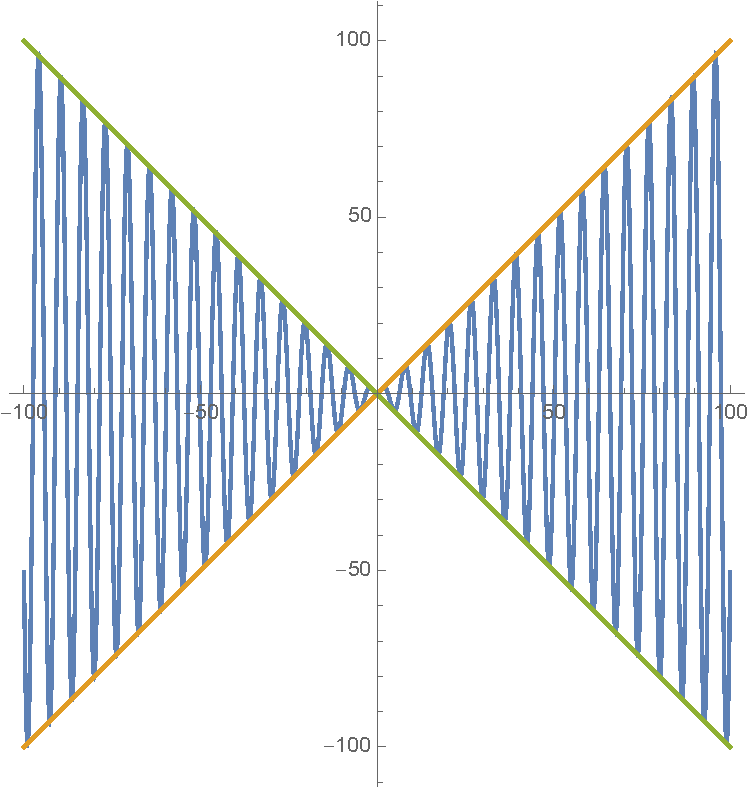
\includegraphics{./images/ch1/xsinx.pdf}}
		\resizebox{!}{3cm}{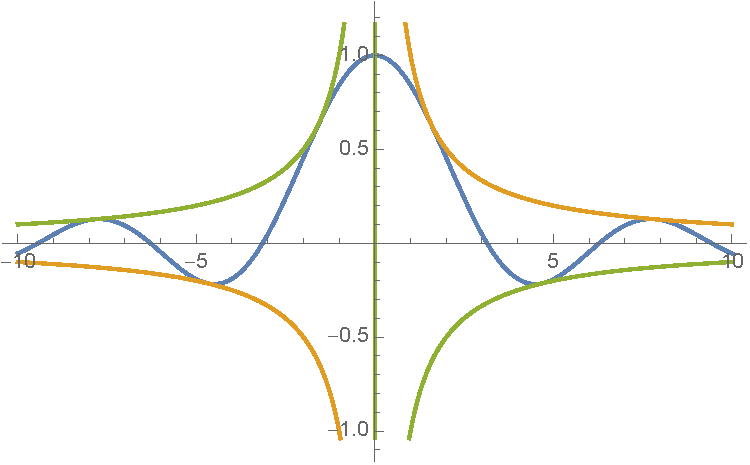
\includegraphics{./images/ch1/1xsinx.pdf}}	
		\resizebox{!}{3cm}{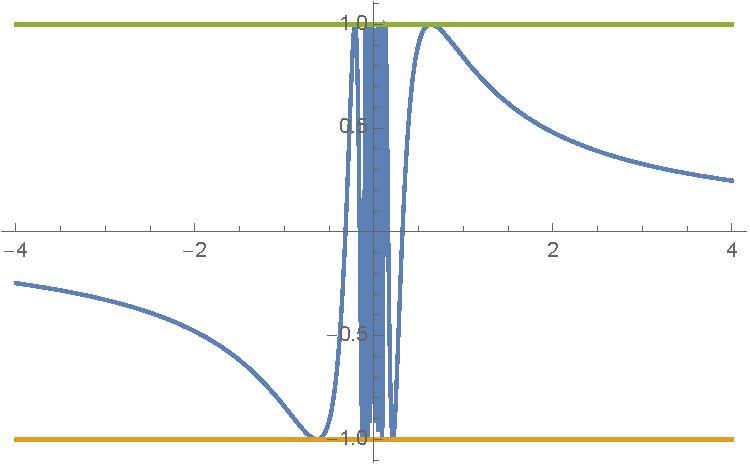
\includegraphics{./images/ch1/sin1x.pdf}}
	\end{center}
	
\begin{shaded}
	{\bf “反面定义”(否命题)的写法*}
	\begin{enumerate}
	  \item {\b “任意”与“存在”互换}
	  \item {\b “$\geq(\leq)$”与“$<(>)$”互换}
	  \item {\b “和”与“或”互换}
	\end{enumerate}
	
% 	[提示]::参考De Morgen律,任何命题的成立都是与一定范围有关的
	以函数的有界性为例,其否命题为函数无界。
	
	{\bf 定义}(有上界)设函数$f:D\mapsto\mathbb{R}$,若{\b 存在}$M\in\mathbb{R}$,对
	{\b 任意}$x\in D$,有$f(x){\b \leq} M$,则称{\it $f(x)$有上界}。
	
	{\bf 定义}(无上界)
		设函数$f:D\mapsto\mathbb{R}$,若对{\b 任意}$M\in\mathbb{R}$,{\b 存在}$x_M\in
		D$,使得$f(x_M){\b >}M$,则称{\it $f(x)$无上界}。
	
	
	{\b {\bf 例:}证明$y=x\sin x$无界。
	
	{\bf 证:}对任意$M\in\mathbb{R}$,
	令$x_M=\left(\left[\df{M}{2\pi}\right]+1\right)\cdot2\pi+\df{\pi}2$(其中$[x]$为下取整函数),
	则有
	$$x_M>\df{M}{2\pi}\cdot2\pi+\df{\pi}2>M,\quad\mbox{且}\quad \sin x_M=1,$$
	故
	$$x_M\sin x_M=x_M>M.$$
	由函数无上界的定义,可知该函数无上界,从而无界。}
	
	{\bf 思考:}数列极限的反面定义:
	
	{\bf 数列$\{a_n\}$以$A$为极限:}$\limn a_n=A$,当且仅当:任意$\e>0$,存在$N$,对任意
	$n>N$,满足$|a_n-A|<\e$
	
	{\bf 数列$\{a_n\}$不以$A$为极限:}$\limn a_n\ne A$,当且仅当:存在$\e_0>0$,对任意$N$,
	存在$n_0>N$,满足$|a_{n_0}-A|\geq\e_0$
\end{shaded}		

\subsubsection{【单调性】}

{{\bf 定义:}}设$f:I\mapsto\mathbb{R}$,若$\forall x_1,x_2\in I$
$$x_1<x_2\Rightarrow f(x_1)\leq f(x_2)$$
则称{\it $f(x)$在$I$上单调递增}(若不等式中的等号总是无法成立,则称其为严格单调递增)
	
{\b{\bf 例:}证明函数$f(x)=x+\sin x$严格单调递增。}

{\bf 证:}任取$x_1,x_2\in\mathbb{R}$,则
$$f(x_2)-f(x_1)=(x_2-x_1)+2\sin\df{x_2-x_1}{2}\cos\df{x_2+x_1}{2}.$$
若$x_2-x_1>2\pi$,则
$$f(x_2)-f(x_1)>(x_2-x_1)-2>2\pi-2>0,$$
若$0<x_2-x_1<2\pi$,注意到$|\sin x|<x\;(x>0)$,则
$$f(x_2)-f(x_1)>(x_2-x_1)-2\left|\sin\df{x_2-x_1}{2}\right|
>(x_2-x_1)-2\df{x_2-x_1}{2}=0,$$
综上对任意$x_2>x_1$,恒有$f(x_2)-f(x_1)>0$,即$f(x)$严格单调递增。

\begin{center}
	\resizebox{!}{5cm}{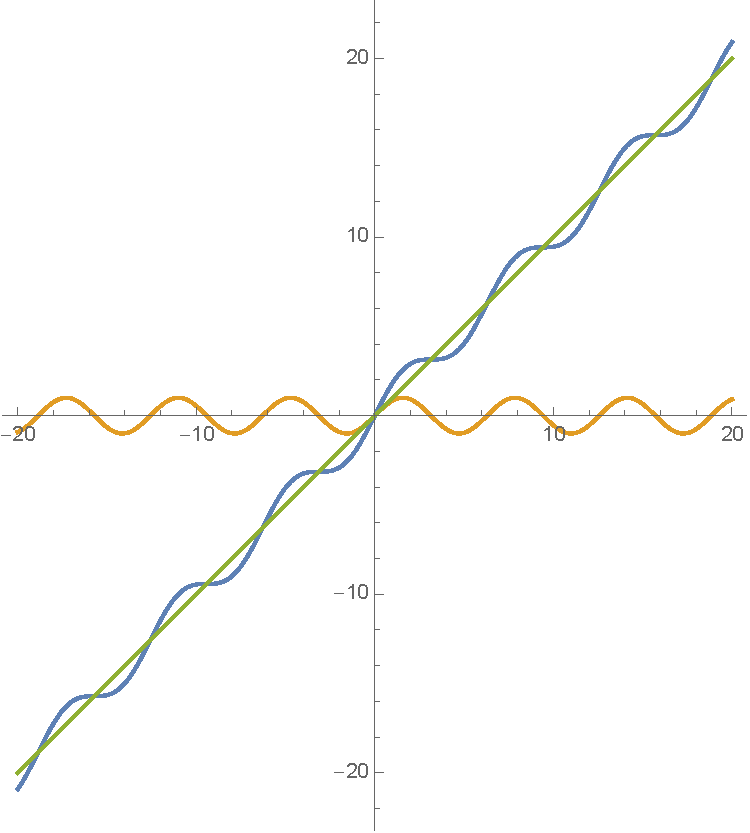
\includegraphics{./images/ch1/xpsinx.pdf}}
\end{center}

{\b{\bf 问:}严格单调的函数一定存在反函数。反之呢?}\ps{要说明一个命题不成立,只需举出反例即可}

{\bf 答:}反之不成立。例如函数
$$f(x)=\left\{\begin{array}{ll}
	x,&0<x<1;\\
	3-x,&1\leq x<2
\end{array}\right.$$
的反函数就是其自身,但在定义域上不是单调的。

{\b {\bf 思考:}若对任意$x_1,x_2$,总有
$$[f(x_2)-f(x_1)](x_2-x_1)\leq 0,$$
则可以推断$y=f(x)$具有何种性质?\hfill({\it 答:$y=f(x)$单调递减})}

\subsubsection{【奇偶性】}

{{\bf 定义:}}
	设函数$f:D\mapsto\mathbb{R}$,
	{\it 称$f(x)$为偶(奇)函数},是指: 对任意$x\in D$,有
	$$f(-x)=f(x)\quad(f(-x)=-f(x))$$

{{\bf 例:}试给出如下性质的数学定义}
\begin{enumerate}[(1)]
  \setlength{\itemindent}{1cm}
  \item {\b 函数$y=f(x)$的图像关于$x=a$对称\quad$\Leftrightarrow f(2a-x)=f(x)$}
  \item {\b 函数$y=f(x)$的图像关于点$(x_0,y_0)$对称\quad$\Leftrightarrow f(2a-x)=2f(a)-f(x)$}
\end{enumerate}

{\b {\bf 思考:}$f(x)=g(a-x),\;(x\in\mathbb{R})$有什么几何意义?

{\bf 答:}{\it $f(x)$和$g(x)$的图像关于$x=a/2$对称!}}

{\bf 例:}$\sin x=\cos(\pi/2-x)$,
故可知$\sin x$和$\cos x$的图像关于$x=\pi/4$对称。

{\bf 性质:}{\b 任意一个定义在对称区间上的函数均可以表示为一个偶函数和一个奇函数的和},即
$$f(x)=\df{f(x)+f(-x)}{2}+\df{f(x)-f(-x)}{2}.$$

{\bf 例:}
$$e^x=\df{e^x+e^{-x}}2+\df{e^x-e^{-x}}2$$

\subsubsection{【周期性】}

{{\bf 定义:}}
设函数$f:\mathbb{R}\to\mathbb{R}$,
称{\it $f(x)$为周期函数},是指: 存在$T>0$,
使对任意$x\in\mathbb{R}$,有
$$f(x+T)=f(x).$$
 满足以上性质的最小正数$T$称为$f(x)$的{\it 最小正周期}
		 
{\bf 注:}若$T$为$f(x)$的一个周期,则任意$n\in\mathbb{Z}$和任意$x\in\mathbb{R}$,满足
$f(x+nT)=f(x)$

\subsection{常用函数}

\subsubsection{【符号函数】}

  $${\b \bm{\mathrm{sgn}}\,x =\left\{
	\begin{array}{rl}
	-1,\;&x<0 \\
	0,\;&x=0 \\
	1,\;&x>0
	\end{array}
  \right.}$$
  {\bf 注:}{\b $|x|=x \cdot\mathrm{sgn} x$}
	

 \subsubsection{【取整函数(阶梯函数)】}

  $${\b y=\left[ \,x\, \right]}$$
  $[\,x\,]$表示小于等于$x$的最大整数

	
{\bf 注:}有时候还有所谓的上取整和下取整函数

{\bf 性质}
\begin{enumerate}[(1)]
  \setlength{\itemindent}{1cm}
  \item {\b $[x]\leq x<[x]+1$}
  \item {\b $[x+1]=[x]+1$}
\end{enumerate}

{{\bf 例:}给出以下曲线的方程}

\begin{center}
	\resizebox{!}{2.5cm}{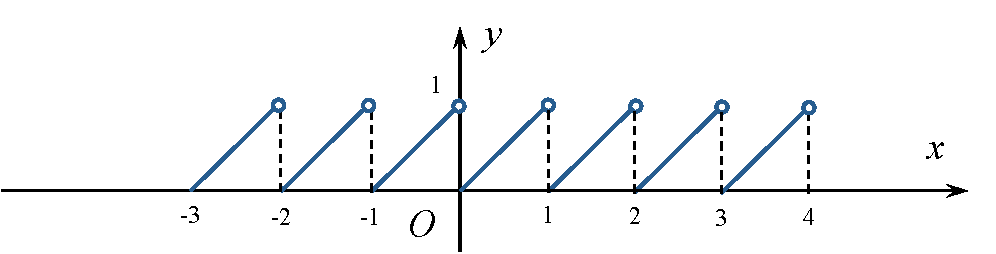
\includegraphics{./images/ch1/f1.pdf}}\quad $x-[x]$\\

	\resizebox{!}{2.5cm}{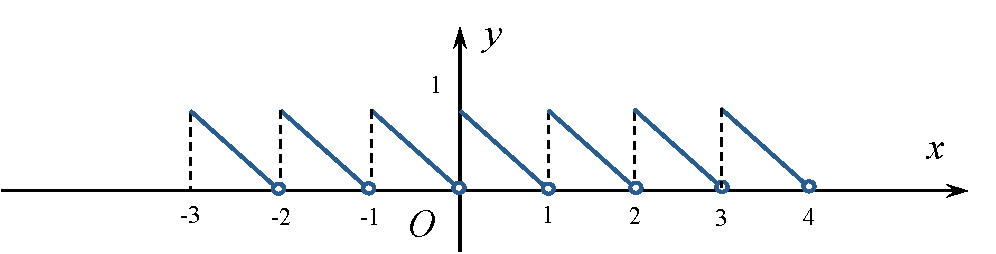
\includegraphics{./images/ch1/f2.pdf}}\quad $[x]-x+1$\\

	\resizebox{!}{2.5cm}{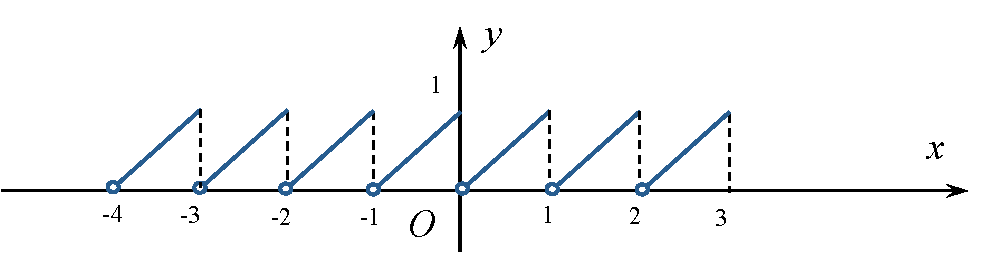
\includegraphics{./images/ch1/f3.pdf}}\quad $[-x]+x-1$
\end{center}
	
{\bf 例:}$(-1)^{[x]}$的图像?\quad({\it 方波!})

{\bf 例:}{\it 三角波}
$$y=\left|x-2\left[\df x2\right]\right|
\quad\mbox{或者}\quad
y=\df1{\pi}\arccos(\cos\pi x)$$

\begin{center}
	\resizebox{!}{2cm}{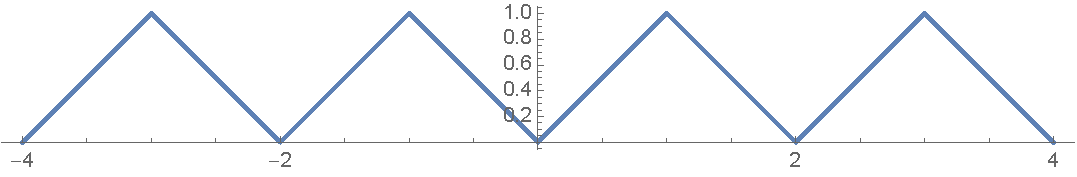
\includegraphics{./images/ch1/trif.pdf}}
\end{center}

{\bf 例:}证明:$f(x)=x-[x]$是以$1$为最小正周期的周期函数。\ps{参见MOOC第四讲}

\subsubsection{【Dirichlet函数】}
  $${\b \bm{D}(x) =\left\{
  \begin{array}{ll}
  	1,\;& x\in\mathbb{Q} \\
  	0,\;& x\notin\mathbb{Q}
  \end{array}
  \right.}$$
  {\bf 性质:}\ps{将在后续章节中加以证明}
  \begin{enumerate}[(1)]
    \setlength{\itemindent}{1cm}
    \item $D(x)$在实数轴上处处无极限
	\item $D(x)$在实数轴上处处不连续
	\item {\it 仅在一点连续的函数:}$y=xD(x)$
	\item {\it 仅在一点可导的函数:}$y=x^2D(x)$
  \end{enumerate}

\subsubsection{【Riemann函数】*:} 

$(x\in[0,1])$
  $$\bm{R}(x) =\left\{
	\begin{array}{ll}
	1,\;&x=0\\
	\displaystyle\frac 1q,\;&x=\displaystyle\frac pq,\,p,q\mbox{互素}\\
	0,\;&x\notin\mathbb{Q}
	\end{array}
  \right. $$
  \begin{itemize}
    \item 对任意$x_0\in[0,1]$, $\lim\limits_{x\to x_0}R(x)=0$
    \vspace{1ex}
    \item $R(x)$在{\it 无理数点连续, 有理数点不连续}
  \end{itemize}

\subsubsection{【初等函数】}

{\bf 五类基本初等函数:}

\begin{enumerate}
  \item {\it 幂函数:} $y=x^a,\; (a\in\mathbb{R})$
  \ps{只有整数次幂的函数可以手工计算!!!}
  \item {\it 指数函数:} $y=a^x,\; (a>0,a\ne 1)$
  \begin{itemize}
    \item {$y=e^x$}
  \end{itemize}
  \item {\it 对数函数:} $y=\log_ax,\; (a>0,a\ne 1)$
  \begin{itemize}
    \item {$y=\ln x$}
  \end{itemize}
  \item {\it 三角函数:} $\sin x, \,\cos x,\, \tan x, \,\cot
  x,\, \sec x,\, \csc x$
  \item {\it 反三角函数:} $\arcsin x, \,\arccos x, \arctan x,
  \ldots$
\end{enumerate}

{\bf 问:}$\arcsin x$和$\arccos x$的定义域值域有何不同?

以上五类函数称为{\it 基本初等函数}。由常数和基本初等函数经过{\it 有限次}的四则
运算和{\it 有限次}的函数复合步骤所构成并{\it 可用一个式子表示}的函数,
称为{\it 初等函数}(同济P17)

{\b {\bf 学习要求:}熟练掌握五类基本初等函数的定义、图像、基本性质、各种运算公式(例如:
三角函数的和差化积、积化和差、半(倍)角公式、万能公式;反三角函数的定义域、值域、单调性;
一些常用的不等式,如$e^x-1>x>\ln(x+1)\;(x>0)$、平均值不等式、
$\sin x<x<\tan x\;(x>0)$等等。}

{\bf 例:}写出以下两个函数的表达式\ps{MOOC第五讲例1}
$$\arcsin(\sin x),\quad \sin(\arcsin x)$$

{\bf 例:}化简$\tan(\arcsin x),\;x\in(-1,1)$\ps{MOOC第五讲例2}

{\bf 解:}注意到
$$\tan x=\df{\sin x}{\cos x}=\df{\sin x}{\sqrt{1-\sin^2x}},$$
故
$$\mbox{原式}=\df x{\sqrt{1-x^2}},\quad x\in(-1,1).$$

\subsubsection{【($n$)次多项式(函数)】}

  {\b $$P_n(x)=\sum_{i=0}^na_ix^i,
  \quad (a_i\in\mathbb{R},a_n\ne 0,i=1,2,\ldots,n)$$
  {\bf 性质:}\ps{掌握结论,不要求了解证明}
  \begin{enumerate}[(1)]
    \setlength{\itemindent}{1cm}
    \item { $n$次多项式方程$P_n(x)=0$在$\mathbb{R}$上最多有$n$个根 (包含重根) ,在
    $\mathbb{C}$上有且仅有$n$个根(包含重根)}
    \item { 设$x_i\in\mathbb{C}(i=1,2,\ldots,n)$为$P_n(x)=0$的全部根 ,则
    $$P_n(x)=a_n\prod_{i=1}^n(x-x_i)=a_n(x-x_1)(x-x_2)\ldots(x-x_n)$$}
    \item { 已知$P_n(x)$在$n+1$个点处的值, 可以唯一确定$P_n(x)$}
  \end{enumerate}
  }

\subsubsection{【有理函数】}

$$f(x)=\frac{P(x)}{Q(x)}, \quad\mbox{其中}P(x),Q(x)\mbox{均为多项式函数}$$
  
{\bf 注:}{\b 任意有理函数总可以化为一个多项式函数和一个真分式(分子的次数比分母低的有理函数)
的和}
	  
{{\bf 例:}用多项式除法化简以下函数}
$$\frac{x^3+x^2-1}{x-1}=x^2+2x+2+\df{1}{x-1}$$
具体的除法过程如下,类似于小学学习过的竖式除法
\begin{center}
	{\b \polylongdiv{x^3+x^2-1}{x-1}}
\end{center}

\subsubsection{【双曲函数】*}

{\small $$\sinh x =\df{e^x-e^{-x}}{2}, \quad
\cosh x =\df{e^x+e^{-x}}{2}, \quad\tanh x=\df{\sinh
x}{\cosh x}, \ldots$$}
{\bf 注:}双曲函数在很多场合也写作$\mathrm{ch}(x)$和$\mathrm{sh}(x)$
\ps{运算规律参见:同济P17-20}

\section{曲线的参数方程和极坐标方程}

{\bf 问题:}$y=f(x)$能否表示平面上的所有曲线?
	
{\bf 或者:}怎样才能更好地表示平面上的曲线?\ps{例如:$x^2+y^2=1,xy=1,x=y^2,\ldots$}

\begin{shaded}
	\begin{center}
		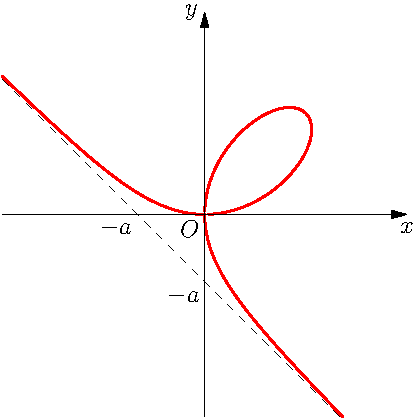
\includegraphics[width=5.5cm]{./images/ch1/dicartesCurve.pdf}

		{\bf Descartes叶形线}
	\end{center}
	\bigskip
	\begin{itemize}
	  \item {\bf 参数方程:}
	  	$$\left\{\begin{array}{l}
	  		x=\df{3at}{1+t^3},\\[1em] y=\df{3at^2}{1+t^3}
	  	\end{array}\right.\;(t\in\mathbb{R})$$
	  	\vspace{-1em}
	  \item {\bf 隐函数方程:}
	  	$$x^3+y^3-3axy=0$$
	\end{itemize}
\end{shaded}

{\bf 例:}求过平面上两点$P_i(x_i,y_i)\,(i=1,2)$的直线方程
		  
$$k=\df{y_2-y_1}{x_2-x_1}=\df{y_2-y_1}{x_2-x_1}$$
由此可给出直线的平面直角方程。若参数化
$$\df{y_2-y_1}{y_2-y_1}=\df{x_2-x_1}{x_2-x_1}=t$$
则有
$$y=ty_2+(1-t)y_1,\quad x=tx_2+(1-t)x_1,\quad (t\in\mathbb{R})$$
		  
{\b {\bf 注:}
\begin{itemize}
  \setlength{\itemindent}{1cm}
  \item 参数方程必须标明参数的取值范围!!!
  \item {利用参数方程可以表示平面上的任意曲线}
  \item {任意曲线的参数方程均不唯一}
\end{itemize}
}

\subsubsection{【极坐标】}

$$(x,y)\;\to\;(\rho\cos\theta,\rho\sin\theta)\quad
(\rho>0,\theta\in\mathbb{R})$$
其中
$$x=\rho\cos\theta,\quad y=\rho\sin\theta,$$
或者反之(假设$\theta\in(-\pi,\pi]$)
$$\rho=\sqrt{x^2+y^2},\quad 
\theta=\left\{\begin{array}{ll}
	\arctan\df yx,& x>0\\
	\df{\pi}2,& x=0,y>0\\
	-\df{\pi}2,& x=0,y<0\\
	\pi+\arctan\df yx,& x<0,y>0\\
	-\pi+\arctan\df yx,& x<0,y<0\\
	\pi,& x<0,y=0\\
	\mbox{无定义},& x=y=0
\end{array}\right.$$
	
{\bf 例:}求以下曲线的极坐标方程\ps{教材1.3.2节例9}
		
\begin{enumerate}[(1)]
  \setlength{\itemindent}{1cm}
  \item $y=kx,(k\in\mathbb{R})$
  \item $x+y=1$
  \item $x^2+y^2=R^2,\,(R>0)$
  \item $(x^2+y^2)^2=2a^2xy$
\end{enumerate}
	
% {\bf 思考:}将极坐标方程化为平面直角方程应注意些什么?



\newpage

\section*{课后作业}

{\bf 【必作题】}\ps{\b 作业必须写明题目所在章节、页码、题号;教材上的题目和作文可不抄题,其余必须抄题;
书写力求清晰,工整;未作或作错的题目讲评后务必及时订正。}

\begin{itemize}
  \item 注册加入课程网站:https://www.trustie.net/courses/844,邀请码:GQCNW
  \item 写一篇短文,内容及要求如下
  \begin{enumerate}[(1)]
    \item 你的个人介绍,请务必包含如下信息:姓名、性别、年龄、籍贯、中学母校的名字、
    你的高考总成绩(以及当地的满分)、你的高考数学成绩(以及当地的满分),贴上一张个人的照片;
    \item 你的兴趣爱好、特长,或者说,你觉得自己有什么与众不同之处;
    \item 你学习数学的体会,例如:喜欢,不喜欢?喜欢什么样的数学,不喜欢什么样的数学?
    有什么好的学习方法?有什么自己觉得成功的经验,或者有趣的经历(最好与数学有关)?
    \item 你期待中的大学课堂是怎样的?怎么的教与学会对你更有帮助?对老师有什么期待、要求,
    或者建议?
    \item 请至少推荐一本(部、套)你喜欢的书、电影或者其他任何可以通过公共渠道获取到的资料
    (例如:网站、软件、APP、\ldots),说说推荐的理由;
    \item 其他任何你认为值得(可以)与我交流的东西,比如你想问我什么问题;
    \item 除第一条必须包含外,其余内容可自由取舍。
    \item 篇幅:作业纸不少于半页,不多于两页(一张纸)。
  \end{enumerate}
  \item 习题1.1:4(2),10
%   \item 给出P8例6中二维球极投影映射中:
%   
%   (1)$Q$的极坐标与$P$的横坐标的对应关系;
%   
%   (2)$Q$的坐标与$P$的坐标的对应关系;
%   
%   (3)描述如何将一个单位球面映射为一个二维平面,给出相应的坐标对应关系。
  \item 习题1.2:3,8,12
  \item 给出教材P20例14中的三角波的函数表达式
  \item 习题1.3:1,5
\end{itemize}

\bigskip

\hrule

\bigskip
\bigskip

{\bf 【思考题】}\ps{\b 思考题主要作为课后的辅助阅读,欢迎课间找我讨论,不必写在作业纸上}

\begin{itemize}
%   \item 习题1.1:(C)应用题
  \item 习题1.2:13,17,22,23
  \item 习题1.3:6,7,9
  \item 习题5.2:3
  \item 阅读:李开复,《给未来的你》
\end{itemize}

\newpage

\section*{部分习题参考解答}

1. 习题1.1:10,证明:
$$\df{a_1+a_2+\cdots+a_n}n\geq\sqrt[n]{a_1a_2\cdots a_n},$$
其中$a_i(i=1,2,\ldots,n)$均为非负实数。

证法一:易证$n=2$时不等式成立。假设对$n=2^k(k\in\mathbb{Z}_+)$不等式成立,则
当$n=2^{k+1}$时,
\begin{eqnarray*}
	a_1+a_2+\cdots+a_{2^{k+1}}&\leq&2^k\sqrt[2^k]{a_1a_2\cdots a_{2^k}}
	+2^k\sqrt[2^k]{a_{2^k+1}+a_{2^k+2}+\cdots+a_{2^{k+1}}}\\
	&\geq&2\cdot 2^k\sqrt{\sqrt[2^k]{a_1a_2\cdots a_{2^k}}\cdot
	\sqrt[2^k]{a_{2^k+1}+a_{2^k+2}+\cdots+a_{2^{k+1}}}}\\
	&=&2^{k+1}\sqrt[2^{k+1}]{a_1a_2\cdots a_{2^{k+1}}}
\end{eqnarray*}
由数学归纳法,可知当$n$取$2$的整数次幂时,不等式成立。

若$n$不等于$2$
的某个整数次幂,不妨设$2^{k-1}<n<2^k(k\in\mathbb{N})$,于是
\begin{eqnarray*}
	& &a_1+a_2+\cdots+a_n+\left(2^k-n\right)\sqrt[n]{a_1a_2\cdots a_n}\\
	& & \quad\geq 2^k\sqrt[2^k]{a_1a_2\cdots a_n\left(\sqrt[n]{a_1a_2\cdots
	a_n}\right)^{2^k-n}}\\
	& &\quad =2^k\sqrt[n]{a_1a_2\cdots a_n}
\end{eqnarray*}
以上不等式稍加整理即证。

证法二:易证$n=2$时不等式成立。以下假设$n=k$时不等式也成立,即
$$\df{a_1+a_2+\cdots+a_k}{k}\geq\sqrt[k]{a_1a_2\cdots a_k}.$$
当$n=k+1$时,记$t=a_1+a_2+\cdots+a_k$,且不妨设$a_{k+1}=\max\{a_1,a_2,
\cdots,a_{k+1}\}$,即$ka_{k+1}\geq t$,也是
\begin{eqnarray*}
	\left(\df{a_1+a_2+\cdots+a_{k+1}}{k+1}\right)^{k+1}
	&=&\left(\df{t+a_{k+1}}{k+1}\right)^{k+1}
	=\left[\df tk+\df{ka_{k+1}-t}{k(k+1)}\right]^{k+1}\\
	&\geq&C_{k+1}^0\left(\df tk\right)^{k+1}+C_{k+1}^1\left(\df tk\right)^k
	\df{ka_{k+1}-t}{k(k+1)}\\
	&=&\left(\df tk\right)^ka_{k+1}\geq a_1a_2\cdots a_{k+1}
\end{eqnarray*}
即证。
\bigskip

2.给出P9例6中二维球极投影映射中:
  
(1)$Q$的极坐标与$P$的横坐标的对应关系;
  
(2)$Q$的坐标与$P$的坐标的对应关系;
  
(3)描述如何将一个单位球面映射为一个二维平面,给出相应的坐标对应关系。

解:
\begin{center}
	\resizebox{!}{5cm}{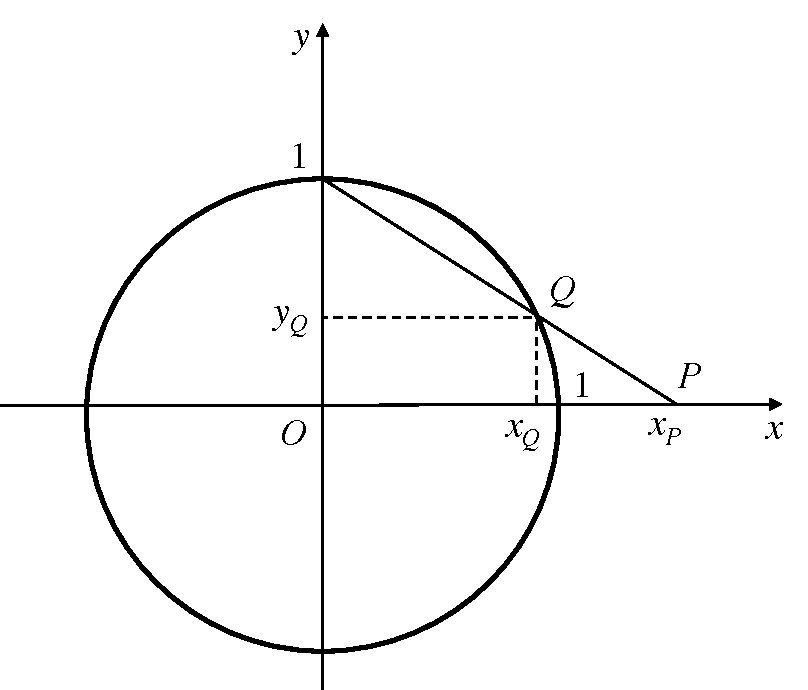
\includegraphics{./images/ch1/answer/sphereline2D.pdf}}\quad
	\resizebox{!}{5cm}{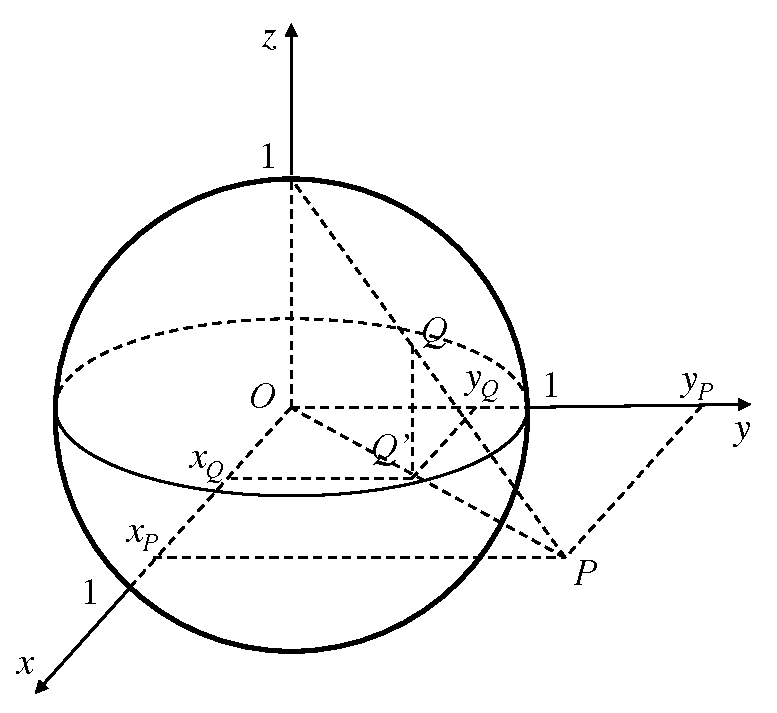
\includegraphics{./images/ch1/answer/sphereline3D.pdf}}
\end{center}
(1)(2) 如左图,设$P,Q$的坐标分别$(x_P,0),(x_Q,y_Q)$,则有
$$
\left\{
\begin{array}{l}
	x^2_Q+y^2_Q=1\\
	\df{x_Q}{x_P}+y_Q=1
\end{array}
\right.
$$
由此可解得
$$y_Q=\df{x^2_P-1}{1+x^2_P},\quad x_Q=\df{2x_P}{1+x^2_P}.$$
进而可知$Q$的极坐标为$(1,\theta)$,其中
$$\theta=
\left\{
\begin{array}{ll}
	\arccos\df{x^2_P-1}{1+x^2_P},& x_P\geq 0\\
	\pi-\arctan\df{x^2_P-1}{1+x^2_P}, & x_P<0
\end{array}
\right.
$$
(3)如右图,设$P,Q$的坐标分别$(x_P,y_P,0),(x_Q,y_Q,z_Q)$,则有
$$
\left\{
\begin{array}{l}
	x^2_Q+y^2_Q+z^2_Q=1\\
	\df{x_Q}{x_P}=\df{y_Q}{y_P}=1-z_Q
\end{array}
\right.
$$
由此可解得
$$
\left\{
\begin{array}{l}
	x_Q=\df{2x_P(x^2_P+y^2_P)}{1+x^2_P+y^2_P}\\
	y_Q=\df{2y_P(x^2_P+y^2_P)}{1+x^2_P+y^2_P}\\
	z_Q=\df{1-x^2_P-y^2_P}{1+x^2_P+y^2_P}
\end{array}
\right.
$$

\bigskip

3.习题1.2:8,题略

\begin{center}
	\resizebox{!}{5cm}{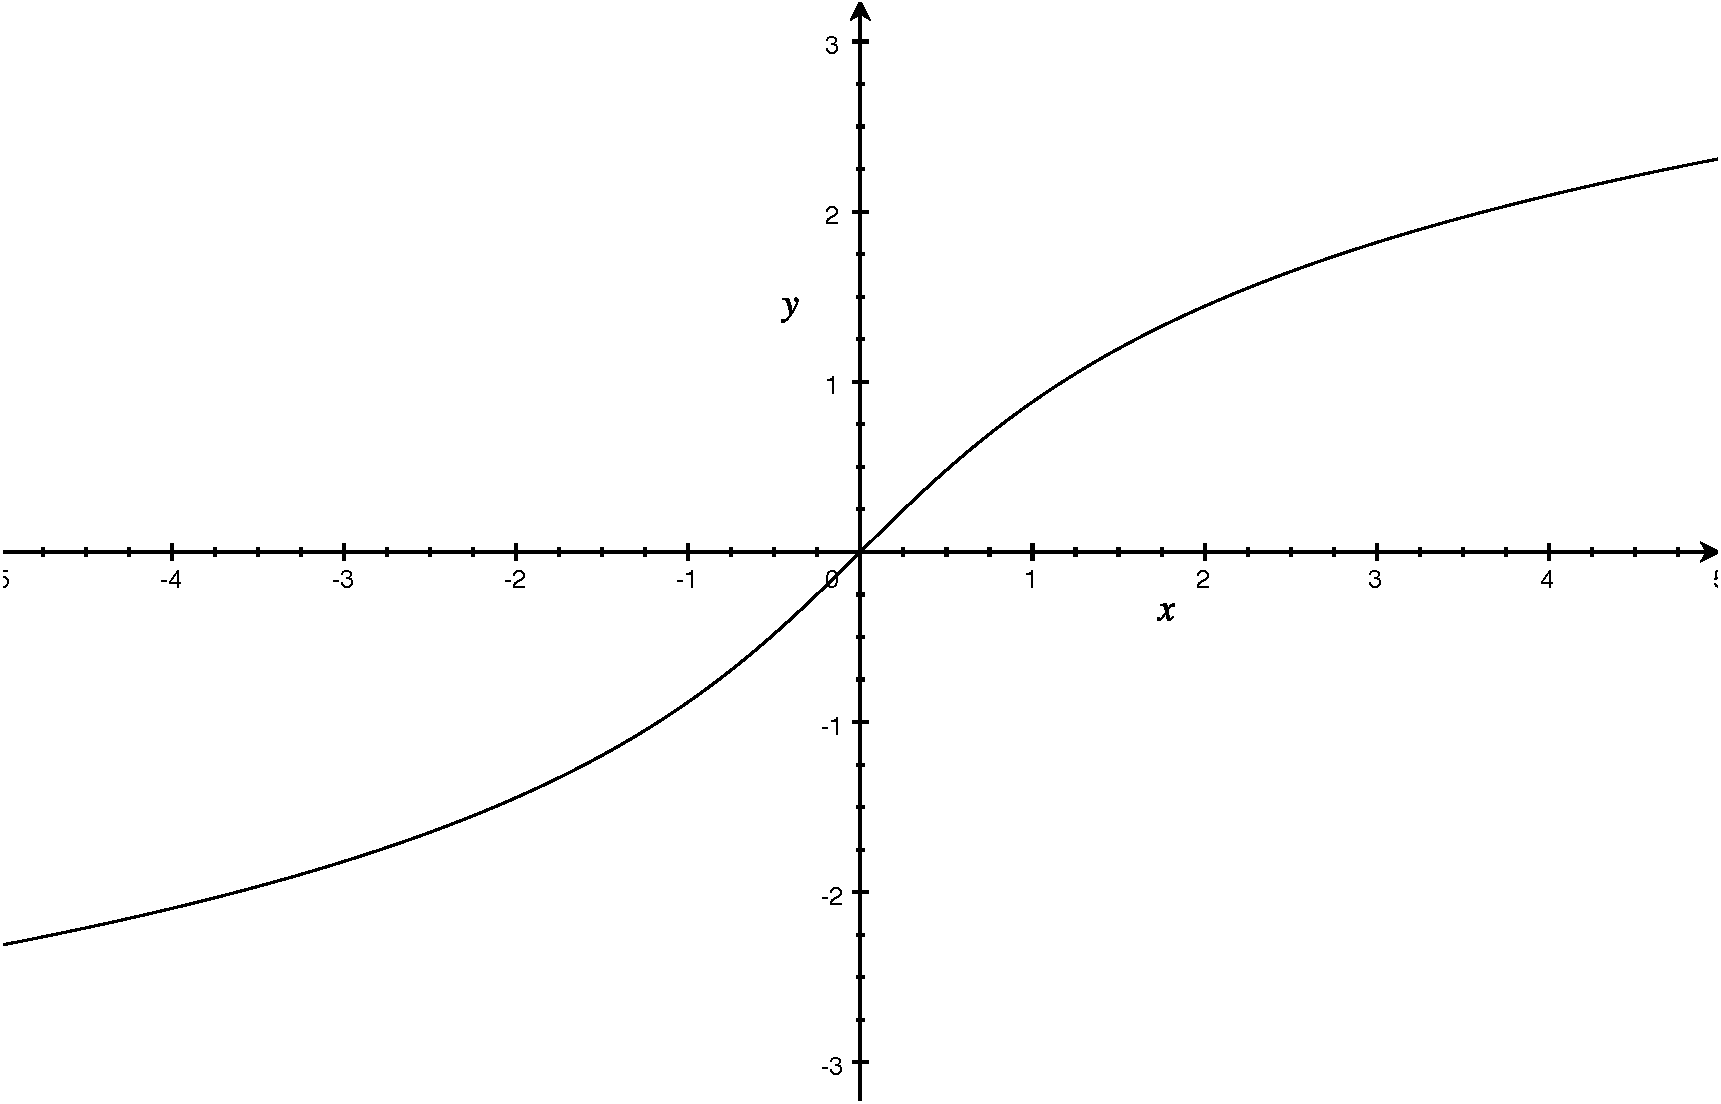
\includegraphics{./images/ch1/answer/lx.pdf}}
	
	$y=\ln(x+\sqrt{1+x^2})$的函数图像
\end{center}

证明要点:容易验证该函数为奇函数。故若可以证明$x>0$时函数严格单调递增,则可断言
函数整体是严格单调递增的。事实上,设$x_2>x_1>0$,则
\ps{证明中用到的{\b 分子有理化}是处理无理分式的常用技巧}
\begin{align}
	f(x_2)-f(x_1)&=\ln\df{x_2+\sqrt{1+x_2^2}}{x_1+\sqrt{1+x_1^2}}
	=\ln\left(x_2+\sqrt{1+x_2^2}\right)\left(\sqrt{1+x_1^2}-x_1\right)\notag\\
	&>\ln\left(x_1+\sqrt{1+x_1^2}\right)\left(\sqrt{1+x_1^2}-x_1\right)=\ln1=0\notag
\end{align}

\bigskip

4.习题1.2:17,题略

参考答案:
$$f_c(x)=\df12\left(|f(x)+C|-|f(x)-C|\right)$$

\bigskip

5. 习题5.2:3,证明恒等式

(1)$3\arccos x-\arccos(3x-4x^3)=\pi,\left(|x|\leq\df12\right)$

(2)$2\arctan x+\arcsin\df{2x}{1+x^2}=\pi,(x>1)$

证:(1)注意到
$$\cos(3\arccos x)=4[\cos(\arccos x)]^3-3\cos(\arccos
x)=4x^3-3x=\cos[\pi-\arccos(3x-4x^3)].$$
由此可知
$$3\arccos x=2k\pi+\pi-\arccos(3x-4x^3)\quad(k\in\mathbb{Z})$$
或
$$3\arccos x=2k\pi-\pi+\arccos(3x-4x^3)\quad(k\in\mathbb{Z}).$$
容易验证,当$x=0$时后一等式不成立,故只有前一等式成立。
又当$|x|\leq\df12$时,$|3x-4x^3|\leq 1$,进而
$$\pi+\arccos(3x-4x^3)\in[\pi,2\pi],\quad 3\arccos x\in[\pi,2\pi].$$
从而可知必有
$$3\arccos x=\pi+\arccos(3x-4x^3),$$
即证。

(2)由于
$$\sin(2\arctan x)=\df{2\tan(\arctan x)}{1+\tan^2(\arctan
x)}=\df{2x}{1+x^2}=\sin\left(\pi-\arcsin\df{2x}{1+x^2}\right)$$
从而可知
$$2\arctan x=2k\pi+\pi-\arcsin\df{2x}{1+x^2}\quad(k\in\mathbb{Z}).$$
又当$x>1$时,$2\arctan x\in\left(\df{\pi}2,\pi\right),\df{2x}{1+x^2}\in(0,1)$,进而
$$\pi-\arcsin\df{2x}{1+x^2}\in\left(\df{\pi}2,\pi\right),$$
由此可知必有
$$2\arctan x=\pi-\arcsin\df{2x}{1+x^2},$$
即证。

{\bf Note:} Similar equations, like:
$$\df{\pi}4=3\arctan\df14+\arctan\df5{99}$$ 
$$\df{\pi}4=4\arctan\df15+\arctan\df1{239}$$
$$\pi=48\arctan\df1{18}+32\arctan\df1{57}-20\arctan1{239}$$  
noticed that
$$\arctan x=x-\df{x^3}3+\df{x^5}5+\ldots+(-1)^{n+1}\df{x^{2n-1}}{2n-1}
+\ldots,\;x\in[-1,1]$$